\chapter{The Neutral apparatus}
\label{ch:chap2}

The Neutral apparatus was one of the pioneering experiments for the trapping, cooling, and creation of quantum degenerate gases of neutral strontium. As such, there is a plethora of previous theses and publications which extensively outline the details for how to achieve these goals. \hl{refs}. In particular, we refer the reader to the PhD theses of previous Killian lab students: Francisco Camargo, Brian DeSalvo, Mi Yan, Pascal Mickelson, Natali Martinez de Escobar, and Sarah Nagel.

Building upon this previous work, this chapter will forego an extensive review of the basic laser cooling techniques for strontium. 
We refer the reading to the extensive works for a formal discussion of the theory behind laser cooling and trapping.

Instead, we will focus on the systems and processes which are most crucial to the operation of the experiment with an emphasis on technical findings and changes which remain, as of yet mostly, undocumented.

Since it has been 7 years since the last broad apparatus overview and the experiment has grown significantly in complexity, the goal of this chapter is to serve as a reference for future work and students. As such, the following is highly technical and will provide an in-depth review of the operation and current status of the Neutral apparatus.

Where appropriate we will refer the reader to the relevant thesis or published work

Future experiments on the Neutral apparatus aim to explore quantum magnetism using strontium 87 and as such several key changes have been made to the 461 locking and 689 trapping systems which will be detailed below.

Say something about referring to the isotopes by their number for shorthand.

This chapter will begin with a brief overview of our trapping procedure in order to contextulaize the remaining sections which focus on the hardware implementations used.  

\section{Experimental procedure} \label{sec:trapping}

Our experiments begin by cooling and trapping atomic strontium utilizing well-established atomic physics techniques \cite{Metcalf1999,Katori1999,Ido2000,Nagel2003,Mukaiyama2003a,Loftus2004,DeEscobar2009a,Stellmer2009,Stellmer2010,Mickelson2010,DeSalvo2010,Tey2010a}. Fig.\;\ref{fig:energy_level_diagram} shows the simplified energy level diagram employed in our cooling process. Once cooled, we typically obtain bulk samples in an optical dipole trap containing on the order of $10^6$ atoms at temperatures $<1\mu$K and densities between $10^{12} - 10^{15}\,$cm$^{-3}$ depending upon the isotope. Samples of ultracold atoms can then be directly loaded into an optical lattice potential by ramping up the intensity of the laser beams forming the optical lattice.

Reference stellmers thesis, natalis thesis, and pascal for strontium colling and trapping

Brians thesis
refs - [27, 28, 29, 30, 31, 32] for cooling and trapping

This section will outline the experimental procedure followed to laser cool and trap atoms. This process has remained relatively stable throughout the years so we provide only a brief overview and reserve the detailed discussion to the relevant sections following this overview.

that begin nearly every measurement taken on the Neutral machine

 The procedure presented here is generally followed for trapping all isotopes of strontium with the major difference being timescales and of course laser frequencies.

Trapping of the bosonic isotopes of strontium is nearly an identical procedure while fermionic 87 poses a significant challenge due to it high nuclear spin when attempting to cool on the intercombination transition. 

We refer the interested reader to the fermion portion of section 2.7.3 in the PhD thesis of Simon Stellmer for a well written discussion of the relevant physics of trapping 87Sr in the red MOT.

The previous work of Brian DeSalvo on the Neutral apparatus created the first quantum degenerate gas of Sr 87 and interested readers can find a thorough discussion of the nua

Over the time frame of this PhD, we have performed experiments using all four common isotopes of strontium.

In the case of switching 


FRANCISCO
The experiments described in this thesis are performed using ultracold samples of 84Sr in either a thermal or BEC phase. 
To obtain such samples, we go through multiple stages of laser cooling and trapping. 
First, we utilize the 461nm (5s2)1S0 - (5s5p)1P1 broad- line transition to reach 1mK (Fig. 2.1) in a Magneto-Optical Trap (MOT) in combination with a magnetic trap [48]. 
Subsequently we load a narrow-line MOT using the 689nm (5s2)1S0 - (5s5p)3P1 transition cooling down to 2 muK [49]. 
Finally, a recycled-beam optical dipole trap (ODT) [50, 51] is turned on, which can trap millions of atoms at 2mK. 
We conduct experiments at this stage but may also choose to begin an evaporative cooling trajectory which results in BEC samples of several hundred thousand atoms.

Room temperature strontium is a metallic solid. 
As such, we load strontium into an ‘oven- nozzle’ which is heated to 425 C, metallic pellets sublimate resulting in gaseous strontium emitting from the nozzle with a mean velocity of about 450 m/s. 
We achieve trapping of these atoms by employing the 461nm transition in three stages (Fig. 2.2): a 2D-Collimator, a Zeeman Slower, a broad-line MOT (all using the 461 nm, 30.5MHz wide transition). 
Ad- ditionally, there is a decay path to the magnetically trappable 3PJ manifold from the 1P1 line. 
These atoms are collected by the quadrupole MOT field and are repumped back to the ground state for further cooling using the 481nm (5s5p)3P2 - (5p2)3P2 transition.

Immediately following the output of the oven, a 2D-Collimator cools the atoms via optical molasses in the radial direction. 
A retro-reflected beam incident on the atoms in two orthogonal directions perpendicular to the direction of the atom-beam propagation is used. 
By cooling in the transverse direction, we greatly increase the flux of atoms that will enter the trapping region of the MOT. 
We observe approximately an order-of-magnitude increase in the loading rate of the MOT with the inclusion of the 2D-Collimator red-detuned by half the natural linewidth.

Next, the atomic beam enters the Zeeman Slower where the mean axial velocity is reduced from about 450 m/s to about 30 m/s, slow enough for the MOT to capture. 
Using an acousto- optical modulator (AOM), the Zeeman laser beam is red-detuned by 18 times the natural linewidth of the transition in order to avoid scattering in the region of the MOT, therefore a spin-flip configuration is implemented such that somewhere along the path of the Zeeman slower the direction of magnetic field is reversed. 
The relative direction of Zeeman Slower fringe field compared to the on-axis field of the MOT can have a significant impact. 
We find that an anti-parallel configuration is optimal by a factor of apprx 2.

The output of the Zeeman Slower leads to the MOT region. The MOT light is set at a red-detuning of 1.8 times the linewidth of the 461nm transition. 
A large loss channel is present due to decay from the (5s5p)1P1 state to (5s4d)1D2 and subsequently to the (5s5p)3P1,2 states. 
However, the low-field seeking 3P2 states are trapped by the anti-Helmholtz magnetic field of the MOT. 
These atoms can therefore be reintroduced into the main cycling transition by repumping with a 481nm laser to the (5p2)3P2 state. 
Experimentally we find that it is optimal to repump for 50ms after having loaded the magnetic trap for several seconds instead of having the repump beam on during the whole loading procedure. 
Details of the repumping laser can be found in Pakorn Wongwaitayakornkul’s undergraduate thesis. 
For a 2 s load time, this scheme yields 20x106 atoms of 84Sr near the Doppler temperature limit. 
Although 84Sr is the least abundant isotope, at 0.6 perc, and we could instead generate much larger MOT sample with the other isotopes, we chose to use 84Sr for these experiments due to the 123a0 84Sr - 84Sr scattering length, which is ideal for evaporative cooling. 
More details on our broad-line cooling and trapping scheme, including a description of the 461nm laser system, can be found in Ref. [48].

Having produced a trapped gas of ten’s of millions of atoms at about 2mK, the next stage of cooling consistes of a narrow-line MOT. 
Utilizing the (5s2)1S0 - (5s5p)3P1 transition enables us to reach a much colder temperature because of a reduction in line-width of over three orders of magnitude compared to the broad-line MOT. 
The theoretical temperature limits due to the Doppler limit and atom recoil are comparable at about 200 nK, however, experimentally we only cool to about 1 muK which is sufficient to subsequently transfer atoms to the ODT. 
To bridge the gap between broadline MOT and initial ODT temperaures, the narrowline MOT must capture apprx 2mK atoms and cool them to apprx 1 muK. To achieve this, we dynamically change the trap parameters. 
Initially, the narrow-line MOT begins with large laser intensity compared to the saturation intensity, far red-detuning compared to the transition line-width, and a dither of the laser frequency that is also large compared to the line-width. 
This ensures that the initial range of atom velocities at the end of the broad-line MOT will experience cooling and trapping on the 689nm transition. 
As cooling takes effect and temperature falls, these experimental parameters follow suit and are changed to address a narrower velocity distribution, ultimatly yielding apprx 1 muK samples of about two million atoms. 
Details of our narrow-line cooling MOT can be found in Ref. [49].

We load atoms from the narrow-line MOT into a 1064nm infra-red (IR) ODT with two perpendicularly crossed paths (Fig. 2.3). 
Each path is made up of three laser beams co- propagating with 10’s of microns of separation [52], yielding a ‘Top-Hat’ laser profile. 
After loading the Top-Hat ODT, the intensity of the outer two beams linearly decrease to zero over 400ms while maintaining constant intensity in the center. 
At this juncture, apprx 106 atoms at apprx 2 muK are trapped in the ODT and represent a cold thermal sample which we have used for several of our measurements. 
Further cooling via forced evaporation can be employed, which enables an increase in phase-space density sufficient enough to create Bose-Einstein condensates (BEC) of 84Sr [19, 20]. 
We produce samples where 75 perc of trapped atoms are in the BEC phase. Several hundred thousand atoms enter the condensate phase at a peak number density of apprx 4 x 1014 cm-3.

BRIAN
For laser trapping and cooling, we need to work with gaseous Sr, so we begin by heating a sample in an oven up to approx 350C to obtain a significant vapor pressure. 
Directly out of the nozzle, the atoms undergo a stage of two dimensional optical molasses to further collimate the beam. 
After the transverse cooling, the atoms are decelerated in a Zeeman slower to velocities suitable for capture in a magneto-optical trap (MOT). 
These initial cooling stages, and our first stage MOT, utilize the 1S0 1P1 transition in Sr, which requires a laser operating at a wavelength of 461 nm. 
The broad linewidth of the transition results in a large saturation intensity, 40.5 mW/cm2,so laser powers on the order of 100 mW are necessary for the initial cooling stages. 
Our system is based on frequency doubling of IR diode lasers, which can provide the power necessary. 
Laser cooling on the 1S0 1P1 transition is ideal for the initial cooling stage owing to the fast cooling rate and large capture velocity which results from the short lifetime of the excited state and short wavelength of the transition. 
This lifetime yields a broad (30.5 MHz) linewidth. 
However, laser cooling on this transition also comes with the significant drawback that the Doppler temperature is high by ultracold atom standards, TD = 1 mK. 
The lack of nuclear spin in bosonic Sr means that sub-Doppler cooling is not possible in this system. 
Therefore the temperature of the 461 nm MOT cannot be reduced below this limit. 
There is a leak in this transition which we can take advatnage of. 
The 1S0 1P1 transition is not completely closed, and atoms from the 1P1 state can decay via the 1D2 state to the 3P2 state with a probability 16 of 1 x 10-5. 
This state is metastable and has a long lifetime, limited in experiment by blackbody radiation to about 25 s. Within the 3P2 manifold, atoms in low-field seeking mj states can be magnetically trapped by the quadrupole field of the MOT where they remain for their lifetime while being dark to the cooling light [33]. 
The observed 25 s lifetime of this trap is is orders of magnitude longer than the lifetime of the MOT, which allows us to use long loading times.
While the loading rate of atoms into the magnetic trap is clearly reduced compared to the loading rate of the MOT (we need to scatter 105 photons for an atom to end up in the magnetically trapable state), the loss rate is reduced further. 
After this collection phase, the atoms are returned to the ground state via a repumping transition. 
Within the last few years, we have begun repumping along the (5s5p)3P2 - (5p2)3P2 using a 481 nm laser. 
This transition has a few advantages over other schemes used so far for repumping Sr. 
Other schemes include using 497 nm [34] or 3 mum [35], which require expensive laser systems for such an uninteresting purpose. 
Another popular choice is the combination of 707 nm and 679 nm. 
While these are less expensive diode lasers, the requirement of two independent laser systems makes this scheme more complicated than desired. 
By using the (5s5p)3P2 - (5p2)3P2 transition, only a single diode laser is necessary. \hl{say something about isotope shifts of these other repumping transitions?}. 
With the atoms retuned to the ground state, we employ a second MOT operating on the 1S0 -3P1 transition which features a narrow 7.5 kHz linewidth. 
This significantly reduces the Doppler temperature to a few hundred nK and in practice we regularly obtain samples between 1 - 2 muK after 200 ms \hl{change this} of laser cooling. Following this cooling stage, we load atoms into a crossed optical dipole trap (ODT). 
The ODT is derived from a multimode 18 W IPG fiber laser at 1064 nm. \hl{add footnote about this laser dying}.
After an a period of free evaporation being held in the ODT, we begin evaporative cooling for to produce our final sample of ultracold or quantum degenerate gases.
The end of the evaporation typically marks the beginning of the experimental phase and the divergence of our protocol into the specific procedures necessary. 
These may include ramping or pulsing on lattice beams, exciting a collective mode, probing the gas with PAS laser, shelving, etc. 
Once we have completed the experimental phase, we perform absorption imaging along the strong 461 nm transition to determine the characteristics of the gas. 
Typically we perform absorption imaging following a time-of-flight so as to measure both the atom number and temperature at the time of release. 
However, this is not strictly necessary and certain experiments may result in low atomic densities which are not amenable to a time-of-flight due to their low optical depth.

NATALI
Atoms in the 3P2 state (8.3 min. lifetime [77]), however, can be trapped by the quadrupole field of the MOT [78, 79, 80, 65] where they do not scatter 461 nm light. As the 461 nm MOT cooling stage continues, atoms keep accumulating in the 3P2 dark state.

\subsection{Characteristic trapping performance} \label{sec:benchmark_trapping}

The following subsections outline typical trapping parameters and performance for each isotope. Note, that while we have demonstrated the ability to dual trap 84 and 87, full characterization and optimization of this process is currently the subject of future research.

\paragraph{$^{84}$Sr} \label{sec:84_trapping}

Timing diagram
	Blue MOT
	Repump
	Broadband red MOT
	Single Freq red MOT
	IR loading
	Evaporation: typically around 1 to 7s
	Time of flight
	Imaging
Typical settings table
Performance table

\paragraph{$^{86}$Sr} \label{sec:86_trapping}

\paragraph{$^{87}$Sr} \label{sec:87_trapping}


Remember the switch to single frequency

What about values for the experiments?

\hl{would like to put a timing diagram here showing a typical timing sequence for 84, 86, and 87}

Where the heck does that calibration for the MOT coils come from??



\section{Vacuum system and atom source} \label{sec:vac}
	
The Neutral apparatus is built around a stainless steel chamber positioned above the table to facilitate optical access. 
Details on the original construction can be found in Natali's thesis so this section is mainly devoted to covering the few changes which have occured in the intervening years.

Figure \hl{something} shows a complete overview of the chamber assembly. 
The vacuum system can be decomposed into several subcomponents. 
From left to right, the system starts with an oven source based around a custom nozzle design, we have a 6 way tee as the main body for the atom source, a 2D coliamtor, and the entry port of the zeeman slower.
There is a differential pumping tube annd needles on he atom source. Throught he zeeman slower we connect to the main chamber which is a custom 304 stainless steel body supported by the cryo tower which is the entry point for the zeeman laser beam and houses an titanium sublimation catridge (Model:??) .
From left to right these we label these
\begin{enumerate}
\item Atom source (assembly of atom oven housed within the source chamber)
\item 2D collimator
\item Zeeman slower
\item Science chamber
\item Cryo tower (housing a Titanium sublimation cartridge)
\end{enumerate}

Additioanlly, Fig.s \hl{something and something} show different views of the Atom source \& 2D collimator and cryo tower. 
Fig \hl{something} defines a coordinate system and directional labels used throughout this thesis. We also show the orientation of various lasers through the science chamber to orient the reader.
Zeeman beam enters through a certain port in the cryo tower.

Companion figures to those shown in Fig hl{above} are also available in Fig \hl{something} with the positions of heater coils and thermocouples labeled and catalogued which were used for a recent bakeout performed in December 2017. 
Appendix \hl{something} covers the process of this bakeout in greater detail.

\paragraph{Ablating strontium off window}




Figs
	Recreate A.49 but with different labels (instead show the laser directions)
	Create an entire side view of apparatus?
	Add assembly views of source and cryo tower
	Nozzle pictures
	
Resolve
	Needle model?


While unchanging during the time of this phd we have learned a number of crucial 

Pressuess within this chamber ar typically of the order blah


	

\noindent Vacuum system is composed of several key components listed below


The original drawings of these components can be found in App. A.10 of \cite{MartinezdeEscolar2010} along with detailed information of the window and ion gauge placements. 
While the source and science chamber have remained mostly unchanged since this publication, several key improvements and events have occurred over the last few years\footnote{As of April 2019, the most up to date CAD drawing for the Neutral apparatus is located at \texttt{KillianDrobo:\textbackslash Neutral\textbackslash Laboratory Systems\textbackslash Vacuum Chamber\textbackslash Neutral Chamber\textbackslash 2017.12.26\_strontiumvacuum35\_latticetable.dwg}. Additionally, please consult the README file located in this folder for further information.}.
Firstly, when moving labs in 2011 a titantium sublimation pump (model?) was installed in the cryo tower which replaced version one of the high vacuum system shown in Fig. A43 of \cite{MartinezdeEscolar2010}. 
Figs blah - blah show an assembled view of the current apparatus with additional views of the cryo tower and source chambers for clarity. 
Additionally, the original atom oven was upgraded to include capillary tubes constructed from AWG-21 hypodermic needles (model??) to further collimate the atomic beam directly out of the oven \cite{Mazurenko2010}. Fig blah shows a view of the oven currently in the Neutral apparatus and the capillary tubes that were added.




First, the atom source was upgraded to included 2$\mu$m capillary tubes \hl{model} to further collimate the atomic beam out 


Description
	very good resource for design considerations of a similar experiment in Francy's masters chapter 3
	Appendix A.10 of Natali's thesis gives specifics about the construction
		the most notable upgrade to the apparatus since Natali's description was the addition of an extensive second layer surrounding the main chamber. The primary purpose was for shaping the optical dipole and lattice traps but due to its proximity to the chamber, nearly every laser which illuminates the atoms is laucnhed from this platform. Details for the construction of this 
Components
	Atom Source
	2D collimator
	Zeeman slower
	main chamber
	Cryo tower
	Pumps
		Ion pumps
		Ti-Sub pump
	Gauges
		Positions?
History
	
%% Paragraphs
Atom source
	Reference
	Description
	
	
Zeeman slower
	Reference
	Description
		constructed by Pascal
		ask francy for refs or in masters?
		
Main chamber
	reference
	description
	Table of ports with windows
	
All the pieces
	Ion pump - model?
	firerod - model?
	atom shutter - model?
	gate valves - model?
	ti sub
	
	
	
	
Lifetime of atoms once we got vacuum back?

Details of the consturction of the vaccuum system are available in \hl{so and so}

The goal of this section is to provide an overview of the most recent history of the vaccuum system as well as to clarify some of the slightly more ambiguous points about what the construction of the apparatus.

Potentially discuss the concerns we've had about the platform and movement between the chamber and the table. THis can lead to the addition of struts tying the chamber to the platform. This remains a source of concern for heating of the atoms particularly in the optical lattice. 

These concerns are exacerbated by an our finding that increased stability came when adding a partial cover over the platform optics for the optical dipole and lattice traps. Although initially meant as a proctective measure, the addition of this cover resulted in a noticable decrease in shot to shot fluctuations of the cloud position after a time of flight. We found that this stability was a result of mitigating air currents due to the closely located ventilaition system meant to mitigate dust acculation on the optical components.

Drawings for the atom source currently in use on the experiment (as of March 2019) are available in the App \hl{vaccuum}. This oven design is labeled "new nozzle summer 2010", and outlines a heat shield that was ultimately abandoned due to lack of a mechanism to secure it to the base flange. This led to the heat shield falling off when attempting to secure the flange in the apparatus. We hypothesized that lack of a heat shield led to uneven distribution of the thermal energy throughout the oven so we undertook the design of a new oven design to address this issue.

In the late fall of 2017 the neutral apparatus had been under vaccuum for approx 6? years and ater extensive testing we determined that we likely ran out of elemental strontium within the atomic source. This led us to breaking vaccuum, reloading strontium, and performing a small bake down procedure to restablish our presssure. ripor to this event we enjoyed lifetimes on the ordr of 25s s measured by background lifetimes measurements within our IR optical dipole trap. Apprximately a year affter this event we have observed lifetimes on the order of approx 15s, the cause of the discrepanacy is currently unknown.
During the time of breaking vaccuum we decided to attempt everal upgrades to the apparatus such as adding a gate valve between the pumping tower and the zeeman window and redesigning the nozzle source to incorporate a heat shield around the heating element to produce a more even heating environemnt along the nozzle
De to timing we did not install the gate valve before re-establishing vaccuum. The hope in doing this upgrade was to provide a better method for replacing the end cap window which the atom source directly points at. During the course of our experiments this window slowly accumulates a thin layer of strontium which may act as a parital mirror and attentuate the crucially important zeeman beam. As a note of interest, it was shared through private communication with professor Killain that pulsed 532 nm light (such as from a q-locked Verdi system used in the Plasma laboratory) might vaporize the strontium off the window and restore any loss in power. Using a test appartus we were able to verify that indeed we can ablate the strontium off of a coated window, as shown in figure something.
This promising test led us to install an optical traversal port, shown in figure, connecting the two labs. Unfortunately, while flashing the verdi on a small section of the neutral experimental window we found that the energy needed to ablate the strontium was accompanied by deformation of the optical surface of the window. We attritbute this to the thicknes of the coating as the key difference between the experiment and the Neutral machine.
With that fun aside, we oder an extra window and the gate valve to replicate the system put in place on the Rydberg appartus so that future needs to repalce the window coul be accomplished by simply back filling the chamber with dry nitrogen or argon, closing the gate valve and simply replacing it quickly without the need to expose the main chamber body to direct atmospheric gas. 

Reudction of the time the window was exposed to hot strontium led us to install a small servo motor driving the valve (model something) and integrate this mechanism into the experimental runtime. This allows the shutter to only be open during the times that we are actively trapping atoms. Details of the servo motor trigger integration into the neuKLEIN control system are available in App \hl{somewhere}.

The second improvement that we attempted was to redesign the nozzle to include a heat shield. A CAD image is shown in figure. Unfortunately, due to the high tolerances of the base flange and surrounding enclosure the machining required for this custom piece was deemed prohibitvely expensive. A prototype was design following the machine drawings available in App \hl{someplace} but was abandoned due to a bend that developed in the tubing which holds the fire rod. 

However, the largest constraint was due to the flange size of 2 3/8" as the basis for the design. This provides very tight confinement and w

What is the model number for the firerod? What were the materials that were used? 

During the course of realignment of having the vaccuum chamber open, we took the opporuntity to replace the atom source with an uncoated window to aid alignment of the zeeman beam through the entire length of the vaccuum system. While doig this we learned that there is a slight angle to the differential pumping tube which separates the atom source chamber from 2D collimation chamber. While we were not able to determine the severity of the misalignment the main symptom of its existence is the partial occlusion and loss of power in the zeeman slowing beam. With an input power of approx. 120 mW before expansion optics and entering the chamber, we measured 60 mW of power transmitted through the window during our testing. Replacement of this differential pumping tube is problematic as it is part of a copper flange held between flanges connecting the aomt source chamber and 2D collimator. This positioning necessitates a drastic and practically infeasible deconstruction of the vaccuum system to replace. Our goal here is simply to inform future students of this issue as we believe it is the primary cause of the much longer load times needed in the Neutral apparatus when compared to the newly designed Rydberg machine.


	\begin{figure}
		\centerline{
		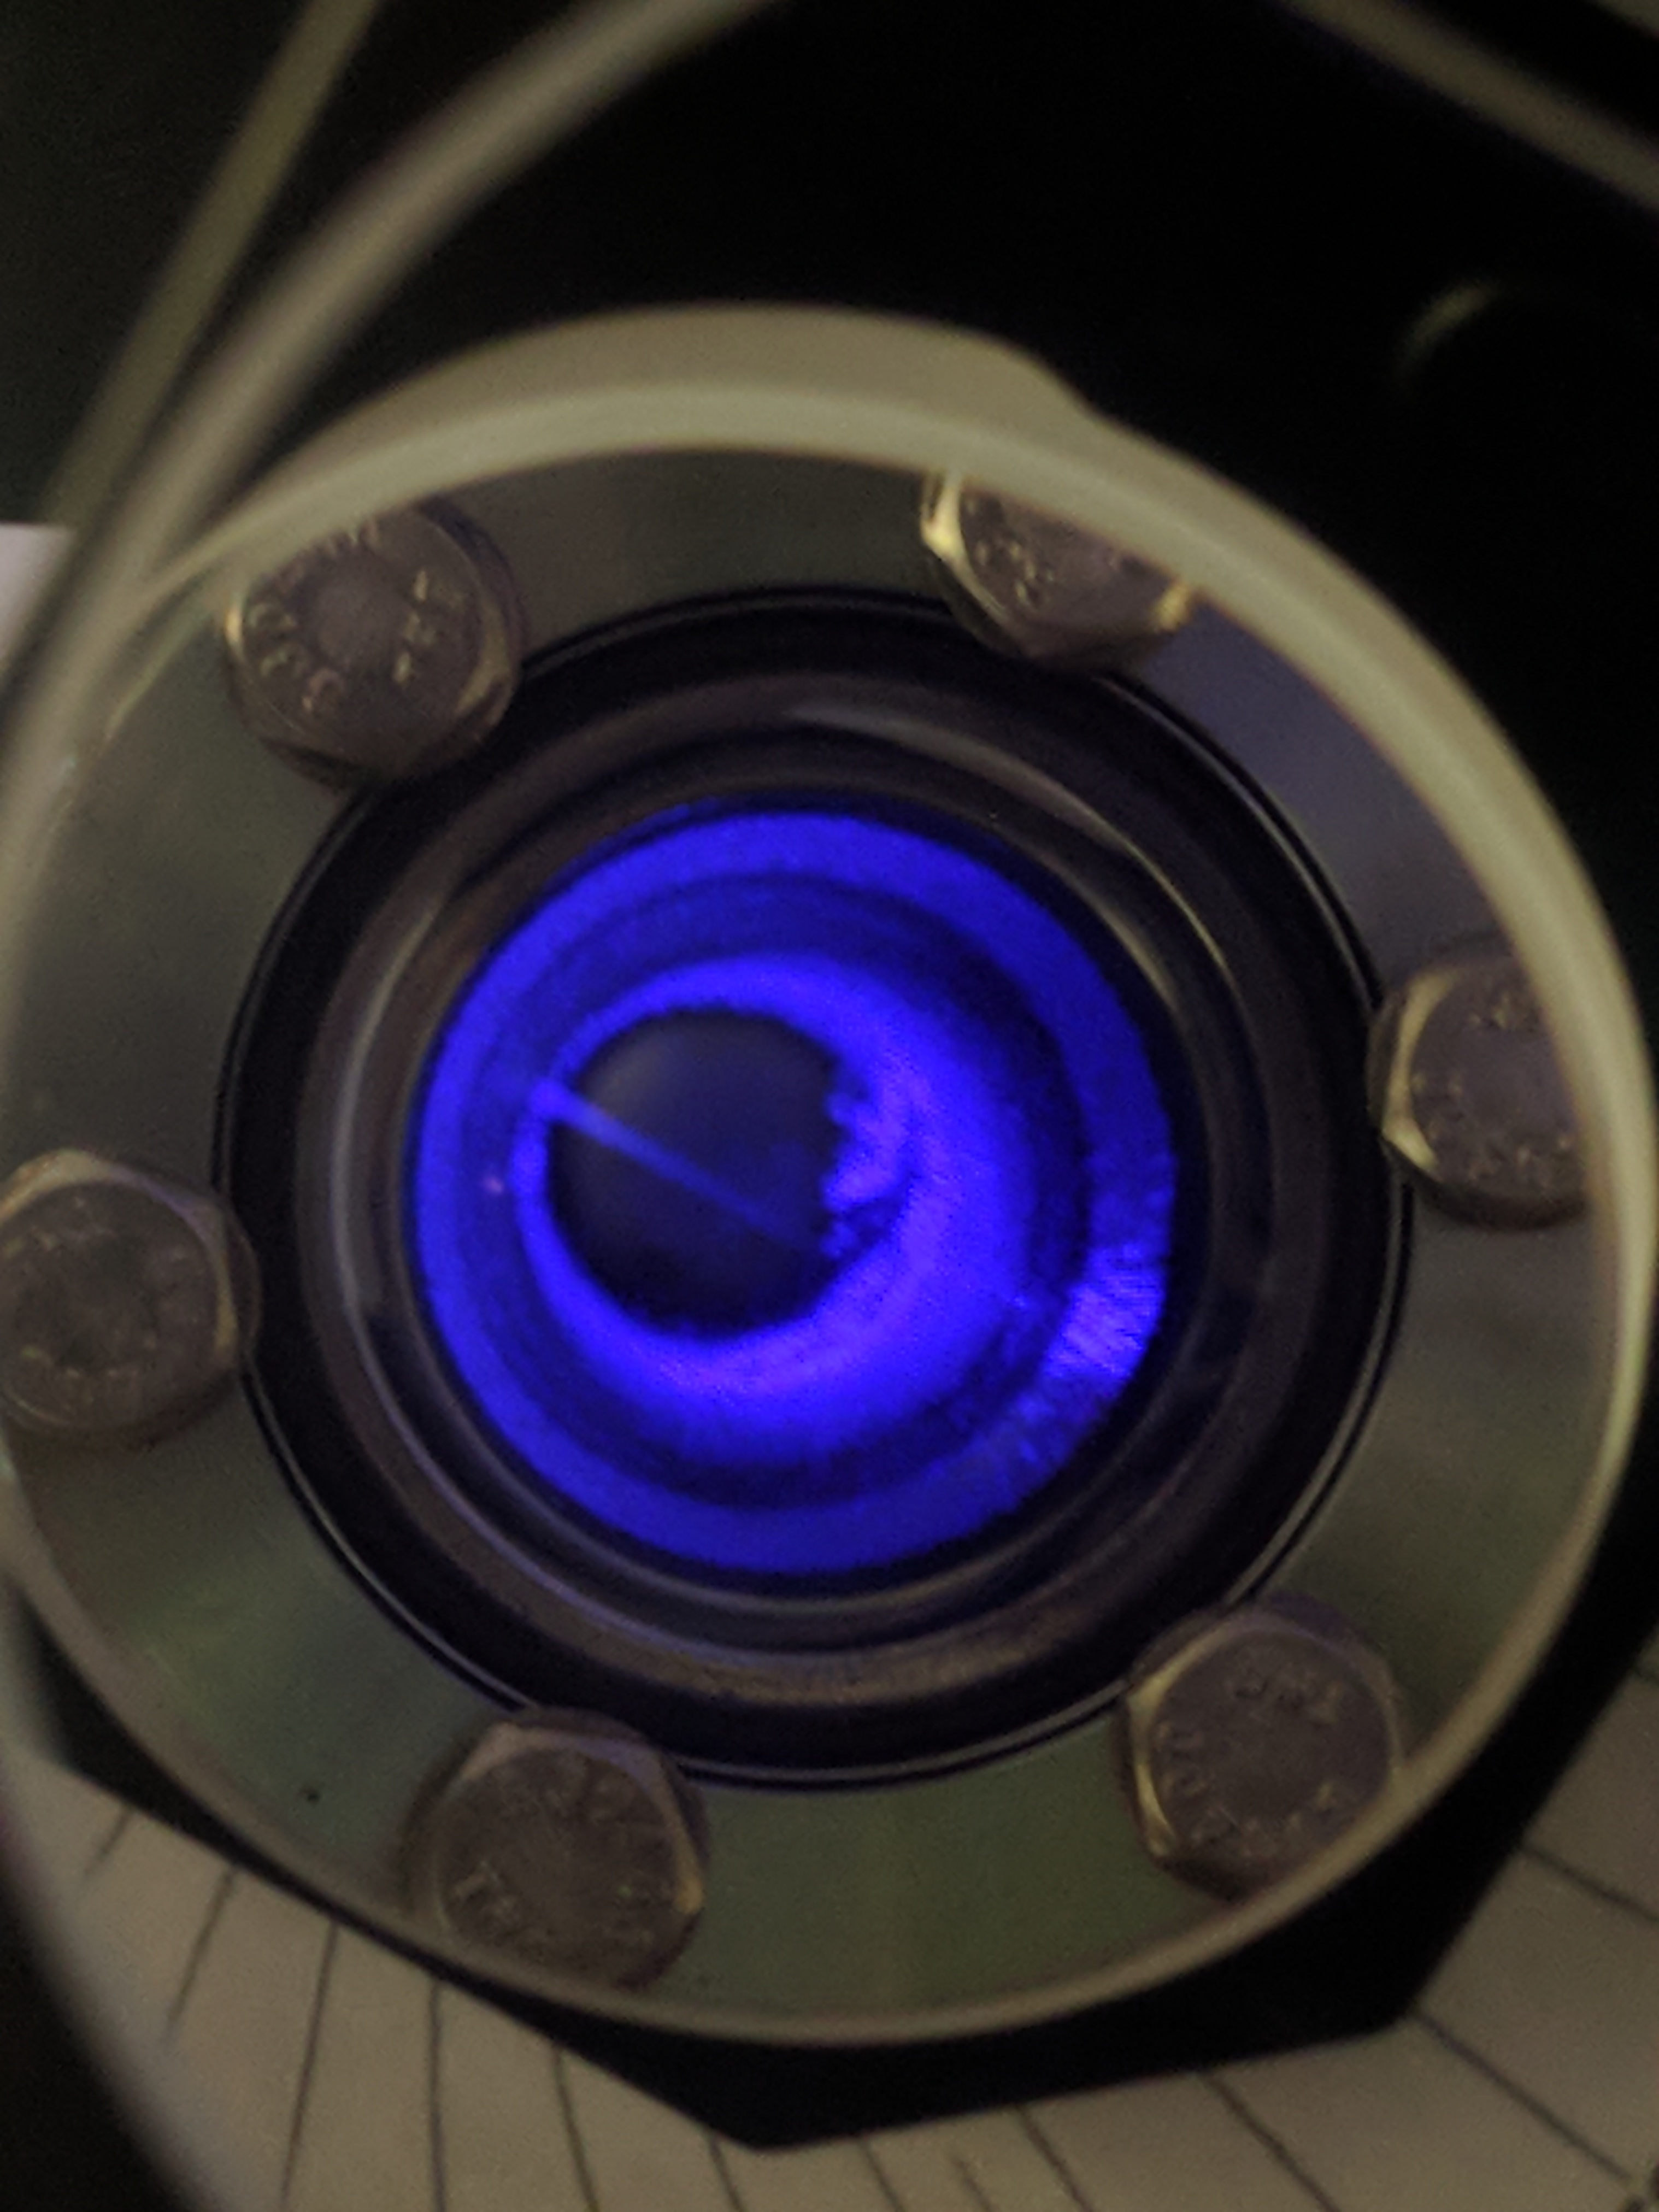
\includegraphics[height=0.75\textheight]{ch_2vacuum_IMG_20171103_184vacuum_230.jpg}}
		\caption{Typical flourescence of Zeeman beam looking down 2D collimator}{This view is found using a 2 in mirror aligned along the path of the first pass of the 2D collimator (near mirror 3 in the diagram), looking down the collimator tube. While looking at this angle, we are able to see the Zeeman beam move across the atom column when moving the last turning mirror. Reduction in this fluorescence signal from that shown was the primary indicator of lack of strontium in the source.}
		\label{fig:2d_coll_flourescence}
	\end{figure} 
	
	\begin{figure}
		\centerline{
		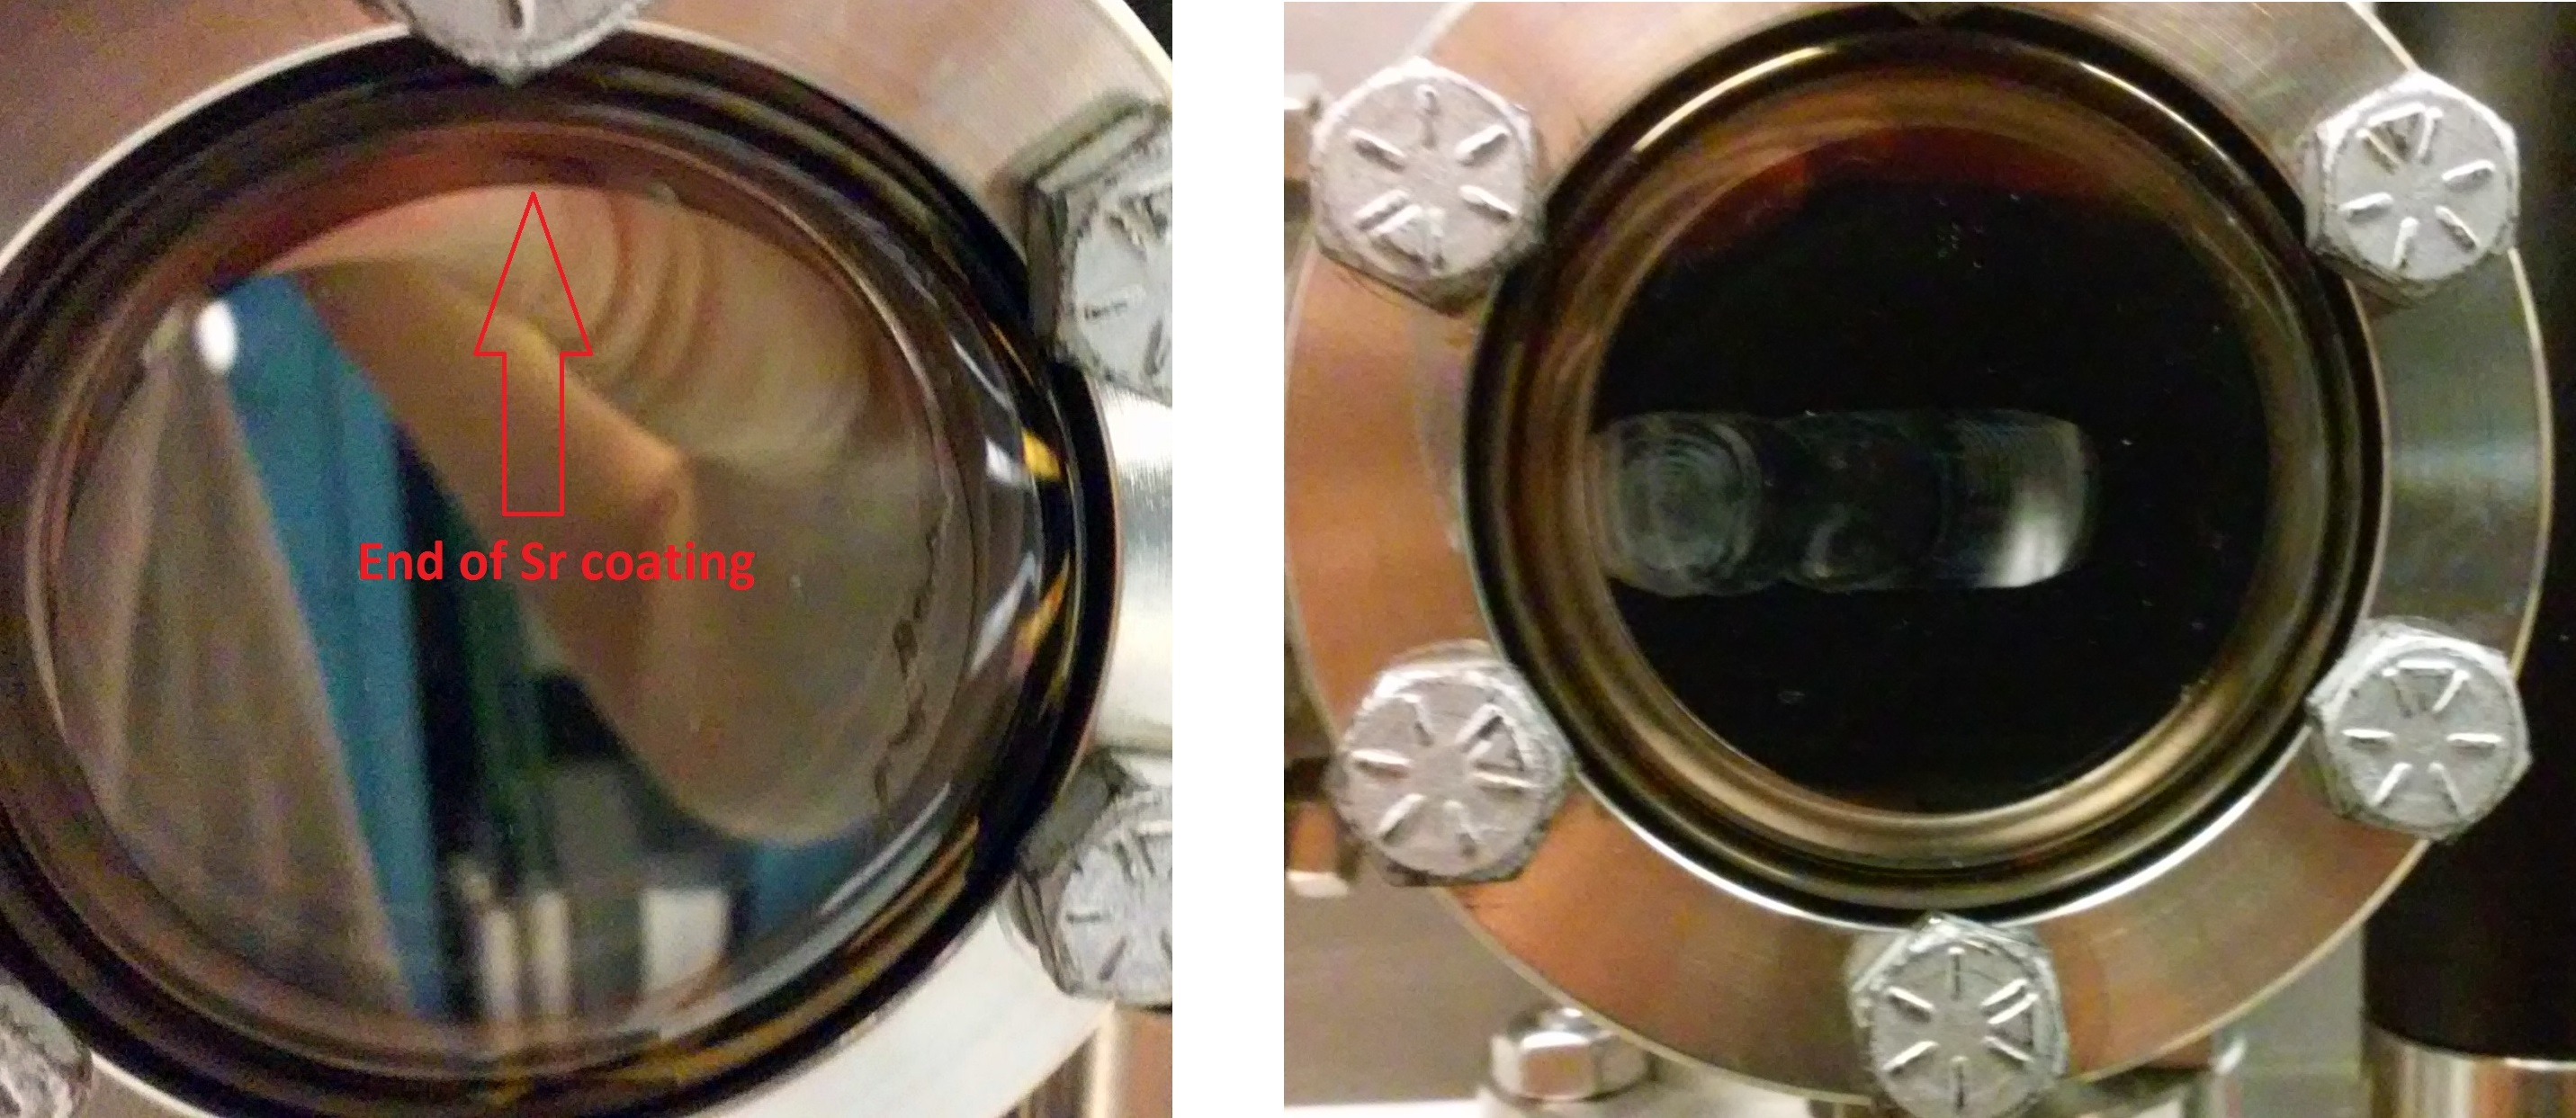
\includegraphics[width=\textwidth]{ch2_ablated_sr2.jpg}}
		\caption{Ablating strontium coating from window}{Comparison of the before (left) and after (right) when using a pulsed 532 nm Verdi to ablate strontium. The residue visible in the after image was due to a higher energy pulse which was reduced as we moved towards the center of the window.}
		\label{fig:ablating_strontium}
	\end{figure} 



\section{Laser systems}\label{sec:laser_systems}

The heart of any atomic physics experiment is the laser systems which can be utilized for various studies. 

Our lab relies heavily upon the use of injection locked lasers \hl{ref}

\subsection{Wideband cooling stage: 461 nm}
\label{ssec:461sys}

\subsubsection{Overview}

The first stage of laser cooling happens on the 1S0 - 1P1 transition which is separated by approx 461 nm. We generate this light by amplifying and frequency doubling 922 nm light.

Generation of 461 nm
	Overview
		isotope shifts
	Components
		922 Master
		MOT light generation
		Zeeman light generation
		Sat Abs
	Diagram

\subsubsection{922 nm master}

The master is a Sacher Lync 922 nm IR diode laser in a Littman Metcalf ECDL configuration. 
As shown in figure something, the light from this diode is shaped and dircted into a fiber optic cable (model?). 

Light is coupled into the fiber, then on the output goes through an AOM which detunes the diffracted order by (how much?). The diffracted and zeroth order are then separated with the unshifted beam sent towards the MOT generation subsystem and the shifted light towards the Zeeman subsystem.

The output of the 922 light has sideband directly on it from a high-pass filter coupled directly to the laser diode.

These sidebands are used to lock perform the PDH lcoking necessary for locking the cavity length. Once 461 nm light has been generated using the MOT subsystem, a small portion is picked off and used to interrogate a saturated absorption cell. Using frequency modulated Doppler-Free saturated absorption we generate an error signal which is used to complete the feedback loop and maintain the frequency position of the complete 461 nm system.
Figure outlines this process.





922 master specifics
	description
	typical running current and temp
	feedback characteristics
	tips of operation
		beware of changing temp
		beware of using the sacher voltage control
	Locking characteristics
		addition of slow lock
			reference that Josh will provide code in his thesis
			note that addition of this slow lock enabled the experiment to stay locked for upwards of 24 hours at a time. As expected, such an increase in stability has greatly improved our ability of taking data.
		main lock circuit
		RF source?
		
\subsubsection{Zeeman subsystem}

Zeeman path
	Description
		construction outlined in chapter 2 of AAron's Saenz's masters thesis
	Components
		TA
		Cavity
		AOMs
		Shutters
	
	Zeeman TA
		Description
			who built
		Components
			Mounts
			Optics
			Circuits
				current control board
				temp control board
					note the thermistor in use
		Typical running values
			in power
			out power
			TA current
			TA temp
		Tips
			power drops occasionally, flip on and off
			alignment can be difficult, try to stabilize in a lower mode
		History
			water got on TA so it might be finicky
		
	Cavity
		Description
			who built
		Components
			Optics
			Circuits
				PDH lock
		Typical running
		Tips

\subsubsection{MOT subsystem}

The MOT path generates light used for a multitude of processes including the first MOT stage, the 2D collimator, the absorption imaging, and the blow away beam, as shown in fig blah. 

MOT light path
	Description
	Components
		TA
		Cavity
		AOMs
		Shutters
	Tips
		advisable to peak up alignment on a daily basis 		
		fairly robust but must keep an eye on as power may fluctuate by as much as 15 percent over the course of a day
	
	MOT TA
		Description
			who built
		Components
			Mounts
			Optics
			Circuits
				current control board
				temp control board
					note the thermistor in use
		Typical running values
			in power
			out power
			TA current
			TA temp
		Tips
		
	Cavity
		Description
			who built
		Components
			Optics
			Circuits
				PDH lock
		Typical running
		Tips


	
	

\subsubsection{Changing isotopes} \label{sssec:change_iso}

The magnetic tunability utilized to control the 461 nm light is well documented in Natali, Pascal, Michael Viray  writeup, others? While the basic setup has not changed over the many year, we have recently moved away from the original current source based on a home built high-current FET amplifier to a Bi-polar something model blah. This change allows for more expansive coverage of the 1S0-1P1 isotopes shifts. The previous current source limited our dual trapping capability of 87+88, and required an AOM to be tweaked and the sat. abs. to be realigned for trapping 84 and 86. Using the BOP we can now span the range of 84 and 87 within a single experimental cycle. However, trapping of 88 still requires the realignment procedure. Care should be taken when adjusting this alignment as the paths are highly coupled as can be seen in Fig \hl{blah}. Below we outline a straightforward algorithm for adjusting this alignment

\begin{enumerate}
\item Change the sat. abs AOM detuning using the potentiometer attached to the sat. abs. VCO. 
\item Peak up the AOM alignment

\end{enumerate}

Using the magnetic tunability of the sat abs as outlined in 

\subsection{Repumping: 481 nm}
\label{ssec:481sys}

Plot from Rydberg

Discuss the change with the EOM
	Frequency center of EOM and range?
	
Data on picking the timescale?
	I know I choose like 40ms (including delay, but did I take data on this)


\subsection{Narrowband cooling stage: 689 nm} \label{ssec:689sys}
\subsubsection{Overview}

Generation of 689 nm
	Overview
	Components
		Toptica Master
		Boson setup
		Fermion setup
		Sat Abs
	Diagram
		AOMs
	
Throughout the course of this PhD, the Neutral 689 nm system has grown significantly and been almost entirely restructured. The master laser system is now shared between the Rydberg and Neutral laboratories and therefore a more modular approach was adopted to ensure independence of the labs experimental schedules. This process began with the replacement of our homemade Littman-Metcalf ECDL 689 master with a Toptica DL-Pro system. Additionally, at the time of this writing (spring 2019) we are currently in the process of migrating from the original high-finesse cavity used for the last 15 years \cite{Nagel2004} of the experiment to an ultra-low expansion cavity system. 

Our new approach to sharing the 689 light is based on fixing the lock point of the 689 light and fibering this fixed frequency light to the separate experiments. From this master fiber we utlize a series of AOM's to choose the correct frequency needed for the experiment at hand. This movement to a fiber based system culminated in the spring of 2018 when the Neutral apparatus significantly refactored our red system and transitioned to an entirely fiber based injection locking scheme. Optical fibers provide several key advantages when used to injection lock slaves, namely a much TEM00 output mode that can be easily mode-matched to the slave. Additionally, fibers provide a quick and effective means for ensuring optimal alignment of the injection locking light by coupling the rejected light from the slave diode "backwards" through the fiber. Although rejected light is typically minimized when setting up a slave diode, by temporarily placing a waveplate before the isolator you can scramble the input polarization and increase the rejected power to facilitate alignment through the fiber. This process generally results in a quite robust alignment of the fiber output and the laser diode and is much faster than the free space method of coupling over a long distance. This alignment advantage along with improved mode matching has allowed us to injection lock a slave diode with as little as 300 $\mu$W while producing up to 24 mW of usable output power.

The rest of this section will detail the setup of the 689 system including the master system and both boson and fermion subsystems used for narrowline cooling and spectroscopy.
	
\subsubsection{689 nm Master}

Description
	Original reference
Diagram
Components
	Mounts
		Riser
	Optics
		Fiber mounts and launchers
	Circuits
		FALC connections
		RF setup
	Systems
		High finesse cavity
		Sat. Abs. 
		Gigahertz AOM
Typical running characteristics
	DLC-Pro settings
	FALC settings
		Figures of linewidth
		measurements of noise
Profiles
Tips for operation
History

\subsubsection{Boson subsystem}

Description
Diagram
	Profiles?
Components
	optics
		isolator
		cubes
		lenses
	mounts
		custom diode holder
	aoms
		RF circuits
	circuits
		temp controller
		current controller
	Spectrum analyzer
		reference?
		refer to the better version developed by Roger
Runnign characteristics
	Example spectrum?
	MOT path powers


\subsubsection{Fermion subsystem}

Discuss the combination of all the paths using the D mirros and how you have to try and do the best you can with alignment. Typically found it best to align beams to center on the cubes and align to the chamber picking one of the paths. Then when adding additional path be careful to only touch the last two mirrors which independetly affect that path.

\paragraph{Stir laser}

Description
Diagram
	Profiles?
Components
	optics
		isolator
		cubes
		lenses
	mounts
		custom diode holder
	aoms
		RF circuits
	circuits
		temp controller
		current controller
	Spectrum analyzer
Runnign characteristics
	Example spectrum?
	MOT path powers

\paragraph{Trap laser}

Description
Diagram
	Profiles?
Components
	optics
		isolator
		cubes
		lenses
	mounts
		custom diode holder
	aoms
		RF circuits
	circuits
		temp controller
		current controller
	Spectrum analyzer
Runnign characteristics
	Example spectrum?
	MOT path powers

\subsection{Optical dipole trap: 1064 nm} \label{ssec:1064sys}

save

Discuss how our only method for evaporative cooling is through light traps since we do not have a magnetically sensitive ground state.

Addres hisotry o laser and say that the current IPg died in fall of last year. 

How much power roughly is split between the arms? AOMs are back to back which couples the power stability of the two arms. This setup allows us to more fully utilize the available power from the IPG and in practice while two completely decoupled independent arms may add a slight complication, when accounted for this has generally not been a major source of concern. We have found it useful though to continously monitor the evaporation trajectory from shot to shot though. As a problem, say with a misbehaving power lock, along one arm may result in intensity fluctuations of both arms.

Several diffferent types of traps have been formed, ref Ying thesis. There are two paths split, named the loading arm and the sheet/dimple arm. Give stats on the loading path The loading path has the ability to be recycled on itself but we have not utilized this capability in many years due to complications of measuring the trap frequencies. 

The sheet/dimple arm can take two configurations as it's name suggests. The sheet trap is an approx. 400 x 40um sheet with the short axis parallel along gravity. This geometry is useful for the low densities needed for Sr 86 to minimize the effecs of three body recombination. Alternatively, by switching out a mirror we can direct this power

Formula for ramp

\subsubsection{Alignment Procedure} \label{sssec:1064_align}

Will focus on independent arm alignment of loading trap and sheet trap

Also useful to imagine three orthogonal axes with their origin set at the center of the chamber.

Need a figure showing the beam prop directions and the setup I'm envisioning.

%% Loading

From the figure, we see that the loading trap propagates primarily along the X-direction. We start by aligning loading trap since it is generally less sensitive and the ports that it goes through are equidistance from the ori

Can generally get away with centering vertically on the chamber windows. 

goal is to rotate about the center point, can verify this by equalizing the distance from the edge of the window on both sides of the chamber

Letting the atoms extend along a single dimension of the trap. 

Moving the red MOT up and down with the z-trim. Dynamic control of z-trim is useful here as you can define a loading b field value then a science b field value.

Use the shortpass dichoric mirrors to counter propagate a red loss beam. Alignment of the red beam follows the usual procedure making sure to reduce the exposure time and power as low as possible while maintaining a loss signal which should maximize alignment.

%%%% Scratch


%%%% Peaking up


%% Sheet

%%%% Scratch

%%%% Peaking up

The sheet trap propagates primarily along the y-axis. This direction has one port extended away from the main chamber body due to the ion gauge. This can complicate the alignment. You

is a little more complicated because it 



For peaking up the the sheet trap alignment, hit the red MOT with the loading trap, then extinguish the red MOT away and hold in the single arm loading trap for approx 10-20ms. This allows the red MOT to fall away and the atoms caught in the ODT will expand along the arm, mapping out the spatial profile. Once the untrapped atoms have fallen away, image the the atoms in situ (i.e. without a time-of-flight). With the spatial profile outlined you should be able to scan the sheet trap vertically looking for horizontal confinement along the loading trap. As the sheet is so tight along the vertical direction, this alignment is done using the last cylindrical lens before the chamber. 

Dimple trap follows the same process as the sheet alignment but there is a Newport Pico motor for finely adjusting instead of a lens.


\subsubsection{Trap frequency calibration} \label{sssec:1064_trap_freq}

Measurement of trap frequencies had previously relied upon parametric heating via intensity modulation of the optical dipole trap \hl{cite Ying thesis}. This process would observe atom loss via resonant heating when the modulation frequency matched a trap oscillation frequency. While this is a convenient and simple process it can lead to quite a complicated spectrum since the heating process does not discriminate directional information and may lead to coupling of higher harmonics of the trap frequencies. 

Cover both methods, moving the laser beam itself and snapping back or using the 532 beam to pull.

Primarily have used the kicking method for the measurement of trap frequencies using independent arm ODT (combination of the loading and sheet/dimple trap). 

With the recent addition of the high power 532 nm for the optical lattice, we have explored an alternative method of inducing a center-of-mass oscillation. This method uses a single pass of the green light purposely misaligned to the equilibrium position of the ODT to pull the atoms and excite an oscillation.

\paragraph{Kicking method}
Primarily have used this For the loading trap. Keep the sheet the 

Use the RF meter to measure the output frequency (eliminates any offset in voltage readings)
Use a dynamic voltage output to load into a trap that is slightly misaligned. Both the 

The process for measuring the horizontal is 
For the current configurations of traps we have found an approx 1 MHz change to the overall RF frequency of 82 (?) MHz to provide a reasonable amplitude. 

Vertical oscillation can be excited by flashing off the sheet trap for 1-2 ms. 

Example time dynamics

\paragraph{Pulling method}

As alluded to above

we have installed an absolute positioning pico motor mirror mount 

\subsubsection{Modeling the potential} \label{sssec:1064_modeling}

Need to discuss this

Give formulas and then approx on harmonic potential and methods for estimating the oscillation freq

\subsection{Optical lattice trap: 532 nm} \label{ssec:532sys}

Brief theory

profiles

Causes for concern
	thermal lensing (both optical power and RF power)
	
Formula for tanh ramp

\subsubsection{Alignment procedure} \label{sssec:532_align}

Porto technique
Lookup note in onenote

Dropping through arm C

\subsubsection{Lattice depth calibration} \label{sssec:532_lattice_depth}

Cover the simple approx and the Gadway method

\subsubsection{Modeling the potential} \label{sssec:532_modeling}

Give the simple forms (plane waves) and the more complete formulas

\subsection{Optical toolbox} \label{ssec:op_tools}

\subsubsection{Absorption imaging system}

Description
Diagram
Components

Give ref to appendix for in-depth technical discussion of image processing

Ref to Mi App A on imaging system

Discuss time of flight pixel calibration as well as the optical magnification system put in place by Mi

Give timing diagram, name the first pulse the atom pulse and the second the background pulse.

Actualy diagram of the imaging system, the light path and the relation of the beam to the chamber

Give reference to section with theory but discuss the technical limitations
 
Absorption imaging is a destructive measurement process which is predicated on measuring the spatially distributed attenuation of laser light after passing through an atomic cloud. In this section we will discuss the technical details of the Neutral absorption system and reserve the theoretical description of the process to Sec.\ref{ssec:tof}. 

We must consider the bit depth of the camera's pixels, which in turn influences the number of photons (the intensity) we can illuminate the cloud with over a certain time. \hl{this must be related to the thinness of the sample right? Thick clouds also mean multiple scatters? Find someone that discusses this idea}.
 
The number of photons needs to be in a certain range, not to little but not too much. \hl{perhaps discuss the real world implication of counting photons (changing the exposure time)} 

This consideration means we generally aim for an optical depth around unity which is an order of magnitude difference the atom and background pulse. 

We use \hl{such and such} camera \hl{include datasheet in appendix since it is hard to find} which has a double shutter function. More details can be found in the appendix \hl{some sec}. We care about the timing since the laser intensity and frequency might drift between the atom and background images. Variations in intensity have straightforward implications for errors since the measurement of the atomic number density assumes the only difference between the images is due to the presence of scatters, Sec.\hl{some sec}, and does not account for fluctuating photon number. Very occasionally, the Neutral apparatus will experience an underexposed shot (of either the atom or background image) that must be discarded due to large, noticeable, fluctuations. We hypothesize that these occurrences are the result of environmental perturbations (acoustic noise, vibrations through the table, spurious ground or electrical noise). However, the precise cause is unknown as the absorption imaging happens very quickly at the end of the experimental cycle when multiple systems begin to reset for the next sequence and in practice, these fluctuations do not occur often enough to be a major cause for concern.

The more insidious source of error in absorption imaging is variation of the optical frequency. Coherent, frequency stabilized radiation is used to illuminate the atom cloud so that we may control the optical absorption cross section and accurately measure the atomic number density. However, this laser light is passed through many optical components on it's path to the atoms and ultimately the imaging camera. Small reflections along this path result in a multitude of interferometers which causes small scale spatial intensity variation across the beam. Exacerbating this problem are short time frequency drifts that may occur between the atom and background images which result in slightly different fringe patterns in the atom and background images. Fringes patterns are a well known nuisance in experimental AMO images and it has become routine to use linear algebra techniques to create a composite background image for each atom image during analysis \cite{Segal2009}. A brief discussion of the principal component analysis (PCA) algorithm employed by the Neutral analysis routine is outlined below, while a more discussion can be found in Sec. \hl{some sec}. Briefly, this approach is as follows:
\begin{enumerate}
\item Find a basis set of background images from a large set of raw background images.
\item For a single atom image, construct an initial guess at a composite background image using coefficients to weight each basis image resulting in a superposition of the basis images.
\item Segment the atom image into multiple regions by separating out the region of interest around the atom cloud.
\item Comparing similar regions between the composite background and the atom background region, perform a least-squares minimization by tweaking the weighting coefficients of the composite background.
\item Once a suitable composite background has been found, calculate the optical depth using the atomic region of interest and the corresponding region of the minimized composite background image.
\end{enumerate}
This procedure is repeated for each atom image using a static background basis set that is periodically recalculated using recent background images to account for long term drifts of the apparatus. may be numerically intensive as it is done for each atom image but the results have proven remarkable for even modest computational resources. 

\hl{add picture showing the fringe removal}

\subsubsection{Chirped blow away pulser}



Reference Josh's master for construction

Reference Natali's(?) thesis for shelving

Discuss usage in measuring Rabi frequencies (add appendix discussing the fitting of the optical bloch equations?)

\subsubsection{Highly tunable 689 nm spectroscopy system}

Discuss all the ways this guy can be injection locked.

Reference Weixuan's writeup. Did he leave a writeup?

Default boson probe beam
	Used for general spectroscopy of 3P1, PAS, and rabi oscillations.
Discuss various configurations and the frequencies resulting in their usage
Bragg beam inputs and reference to Brian’s thesis
Figure - outline various light paths for each config
Outline the inputs and the outputs for the spectroscopy slave


\subsubsection{Spin-manipulation laser with dynamic polarization control}

Outline path, discuss LCR, reference Josh's masters

\section{Experimental control and electronics} \label{sec:electronics}

Huge amount of electronic needed to run this experiment. Primary method of control is analog voltage control or serial connections. 

\subsection{Computer control and measurement system} \label{ssec:comp_sys}

Control
	Pulseblaster for timing
	NI cards for voltage control
		make a table with model number and importnat characteristics
		discuss limitations that must be watched out for
	FPGA system

Measurement
	Pico scope
	pixelfly
	wavemeter

\subsection{Ancillary laboratory systems} \label{ssec:misc_sys}

\subsubsection{MOT coils}

Find reference for circuit

What is the current source

Discuss possible future improvement

\subsubsection{Trim coils}

Standard trim coil apparatus with the coils in a helmholtz configuration.

Used to trim out static residual B-fields and to apply dynamic and well controlled external magnetic fields.

Should include the trim coils in here somewhere and discuss how to zero the B field as well as provide what the calibration factor is for the coils

Model numbers for Gwinstek drivers on Z and Y. Reference something about the BioChip for the X box and give a model number for its current source.

Beware of the high sensitivty of the 3P1 state to B fields. Small changes in current can affect the position of the MOT. Particularly noticable when attempting to zero the field as there may be unknown offsets. It is recommended to 

\subsubsection{Zero crossing AC line trigger}

Give circuit diagram and the logic gates needed to correctly trigger both pulseblasters.

Give data showing that the pulseblasters are synced (if I have it)

\subsubsection{Pneumatic actuated mirror mounts}

Any references?

Diagram
Description
Components
	Circuits
	
